\label{sec:result}
Our experiments aim to investigate the following: (1)~Are density and conservation adversarially related? (2)~How do $\pi$-comparable schemes perform relative to one another under the proposed metric GSS? (3)~Can mask optimization improve the overall performance of both minimizer and syncmer? Through these demonstrations, we confirm our theoretical understanding of various sketching metrics and the relationship among $\pi$-comparable schemes, as well as demonstrate the efficiency of our proposed optimization method. We further conduct ablation studies to investigate several interesting phenomena related to masked minimizers, such as the ability to exploit the relative ordering metric (as mentioned in Section~\ref{sec:metric}); the performance of all masks, which reveals insight on setting a good default mask; and the ability to prevent repeated sampling in a homopolymer-rich sequence, which has previously been a unique advantage of the syncmer method.

\subsubsection{Experimentation details.}  
We compare the following methods to construct the $k$-mer ordering: (1)~random ordering; (2)~training with different variants of the \textsc{DeepMinimizer} loss~\cite{hoang2022deepminimizer}; (3)~constructing the ordering from \textsc{Miniception}~\cite{zheng20miniception}; and (4) \textsc{PASHA} universal hitting sets~\cite{ekim20pasha}. Performance is demonstrated on the following mask parameters: (1) the minimizer mask $\nu = \mathbf{1}_w$; (2) the syncmer mask with offset $t=w/2$ (suggested by Shaw and Yu~\cite{shaw2021theory}) meaning $\nu = \mathbf{e}_{w/2}$; (3) its complement $\nu=\mathbf{1}_w - \mathbf{e}_{w/2}$; and (4) the optimized mask $\nu_\ast$ found by the heuristic search described above. We respectively label the sketches of these masked minimizers as $\mathcal{M}(S),\mathcal{O}_{w/2}(S),\mathcal{C}_{w/2}(S)$ and $\mathcal{V}(S)$. All experiments are trained on human chromosome 1 (labelled \textsc{Chr1}); the centromere region of human chromosome X (labelled \textsc{ChrXC}); and several bacterial genomes that were previously used in Edgar \cite{edgar2021syncmers} (labelled \textsc{Btr1}, \textsc{Btr2}, \textsc{Btr3} and \textsc{Btr4}). The details of these sequences are given in Appendix~\ref{app-mask:d}.
We compute all gradient-based loss functions per batch of sampled subsequences since it is not possible to fit the entire sequence on GPU memory. Other implementation details are given in Appendix~\ref{app-mask:e}. Our implementation can be found at \url{https://github.com/hqminh/maskedminimizer}.
\subsubsection{The adversarial relationship of density and conservation.}
This experiment demonstrates that density and conservation are conflicting objectives for $\pi$-comparable schemes, thus confirming our analysis in Section~\ref{sec:metric}. First, we train masked minimizers for $w=7, k=15$ and various binary masks $\nu$ using three different loss functions: (1)~the \textsc{DeepMinimizer} loss, which only optimizes for density and is labelled as $\mathcal{L}_{DM}$; (2)~only the conservation term in Eq.~\eqref{eq:loss}, which optimizes for conservation and is labelled as $\mathcal{L}_{con}$; and (3)~the combined masked minimizer loss, which is given as Eq.~\eqref{eq:loss} and labelled as $\mathcal{L}_{gss}$. 

\begin{figure}[ht]
\centering
\begin{tabular}{c}
\hspace{-1.7mm}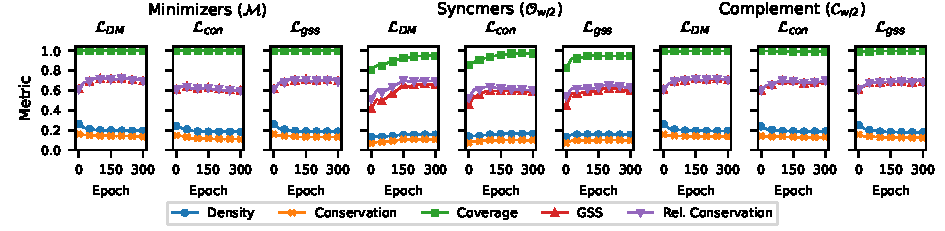
\includegraphics[scale=1.03]{masked_mnz_plots/fig1/w7_k15.pdf}
\end{tabular}    
\caption{Comparing density, conservation, relative conservation and GSS vs. number of training epochs using difference training losses and masks on the bacterial genome \textsc{Btr1}.}
\label{fig:1}
\end{figure}
Fig.~\ref{fig:1} plots the density, conservation, coverage, relative conservation and GSS metrics as these masked minimizer schemes are trained with each loss function over $300$ epochs on \textsc{Btr1}. As predicted in Section~\ref{sec:metric}, we observe that the density metric is consistently greater than the conservation metric in all experiments. Training with any variant of the \textsc{DeepMinimizer} ($\mathcal{L}_{DM}$) loss generally lowers density for minimizer ($\mathcal{M}$) and complement ($\mathcal{C}_{w/2}$) schemes, but also decreases their conservation. On the contrary, the conservation of syncmers ($\mathcal{O}_{w/2}$) increases with training at the expense of raising its density. This is most likely because the sampling behavior of syncmers is not compatible with the above variants of $\mathcal{L}_{DM}$, which was originally designed for minimizers; whereas the complement mask behaves almost identically to the minimizer mask due to its mild sub-sampling.

\begin{figure}[ht]
\centering
\begin{tabular}{cc}
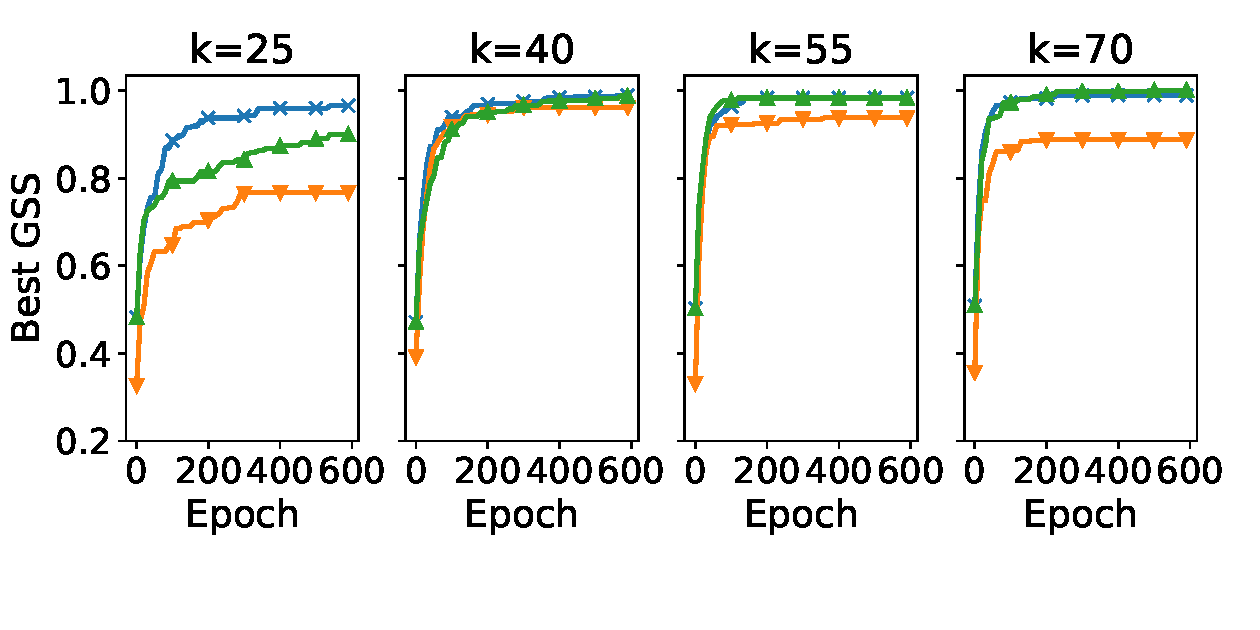
\includegraphics[width=0.487\columnwidth]{masked_mnz_plots/fig2a/compare_best_gss_vs_epoch_chrXC.pdf} & 
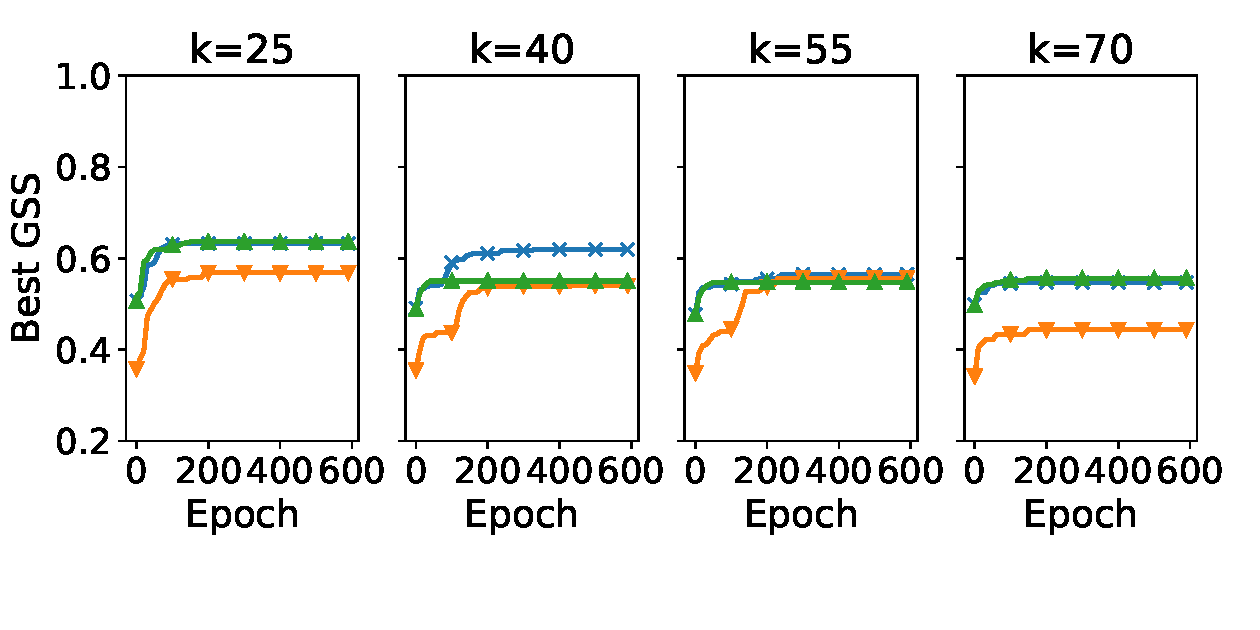
\includegraphics[width=0.487\columnwidth]{masked_mnz_plots/fig2a/compare_best_gss_vs_epoch_chr1.pdf} \\
(a) \textsc{ChrXC}, $w=15$ & (b) \textsc{Chr1}, $w=15$ \\
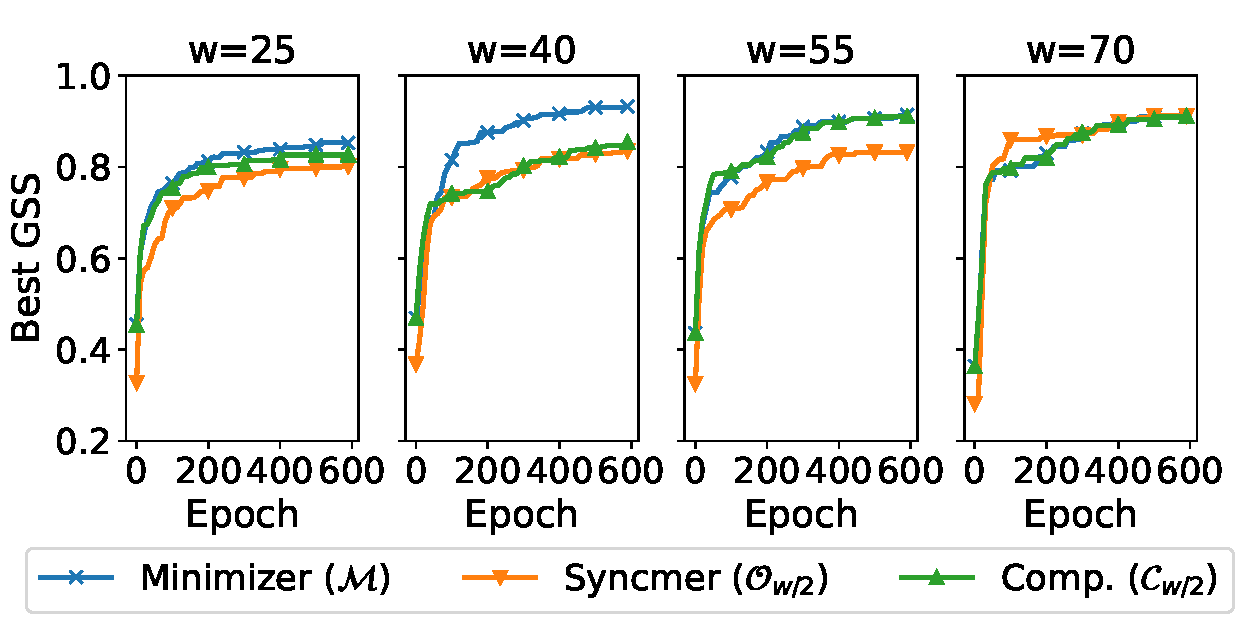
\includegraphics[width=0.487\columnwidth]{masked_mnz_plots/fig2b/compare_best_gss_vs_epoch_chrXC.pdf} & 
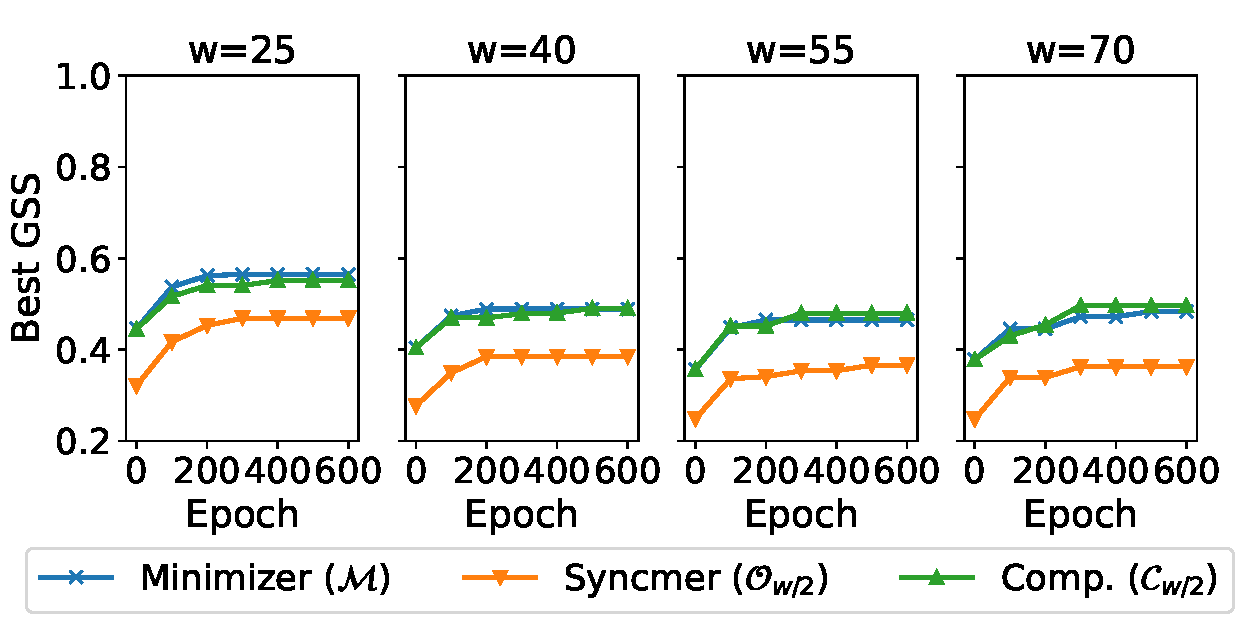
\includegraphics[width=0.487\columnwidth]{masked_mnz_plots/fig2b/compare_best_gss_vs_epoch_chr1.pdf}\\
(c) \textsc{ChrXC}, $k=15$ & (d) \textsc{Chr1}, $k=15$
\end{tabular}    
\caption{Comparing GSS of different masked minimizers vs.\@ number of training epochs on \textsc{ChrXC} and \textsc{Chr1}.}
\label{fig:2}
\end{figure}

\subsubsection{The effectiveness of training masked minimizers.} This experiment demonstrates that our proposed loss function $\mathcal{L}_{gss}$ learns robustly and improves GSS in various settings of $w, k$ and different masks $\nu$. Fig.~\ref{fig:2} plots the GSS of the masked minimizers $\mathcal{M}$, $\mathcal{O}_{w/2}$ and $\mathcal{C}_{w/2}$ over $600$ training epochs in two settings: (1)~$w=15$ and $k \in [25, 40, 55, 70]$; (2)~$k=15$ and $w \in [25, 40, 55, 70]$. This experiment is repeated on two sequences, \textsc{ChrXC} and \textsc{Chr1}. All experiments show that GSS steadily increases over $600$ training epochs by $1.5$ to $5$ times that of their initial random weights. We observe that the performance of minimizers ($\mathcal{M}$) is highly similar to the complement scheme ($\mathcal{C}_{w/2}$), except for $(w,k)=(15,40)$ with \textsc{Chr1} and $(w,k)=(15,25), (40, 15)$ with \textsc{ChrXC}. Both these masks outperform syncmers ($\mathcal{O}_{w/2}$) in most settings, which corroborates the observation in the previous experiment. Appendix~\ref{app-mask:f} shows the individual effects of training on the conservation and density metrics for the experiments in Fig.~\ref{fig:2}(a), thus confirming our analysis in Section~\ref{sec:comparability}.

\newcolumntype{C}{>{\centering\arraybackslash}p{0.8cm}}
\begin{table}[ht]
\begin{center}
\begin{tabular}{CCCCCCCCCCCCC} 
    \toprule
    & \multicolumn{4}{c}{Conservation Loss $\mathcal{L}_{con}$} & \multicolumn{4}{c}{DeepMinimizer Loss $\mathcal{L}_{DM}$} & \multicolumn{4}{c}{Masked Minimizer Loss $\mathcal{L}_{gss}$}
    \\
    \cmidrule(lr){2-5} \cmidrule(lr){6-9} \cmidrule(lr){10-13}
    $(w,k)$ & $\mathcal{M}$ & $\mathcal{O}_{w/2}$ & $\mathcal{C}_{w/2}$ & $\mathcal{V}$ & $\mathcal{M}$ & $\mathcal{O}_{w/2}$ & $\mathcal{C}_{w/2}$ & $\mathcal{V}$ & $\mathcal{M}$ & $\mathcal{O}_{w/2}$ & $\mathcal{C}_{w/2}$ & $\mathcal{V}$
    \\
    \hline 
    $10,10$ & $\textbf{0.701}$ & $0.656$ & $0.685$ & $\textbf{0.701}$ & $0.716$ & $0.529$ & $0.722$ & $\textbf{0.745}$ & $\mathbf{0.754}$ & $0.601$ & $0.753$ & $\textbf{0.754}$ \\
    $10,15$ & $\textbf{0.706}$ & $0.650$ & $0.696$ & $\textbf{0.706}$ & $0.768$ & $0.656$ & $\textbf{0.779}$ & $\textbf{0.779}$ & $0.719$ & $0.566$ & $0.704$ & $\mathbf{0.810}$ \\
    $15,10$ & $0.693$ & $0.621$ & $0.680$ & $\textbf{0.713}$ & $0.690$ & $0.613$ & $0.726$ & $\mathbf{0.765}$ & $0.683$ & $0.597$ & $0.701$ & $\textbf{0.750}$ \\
    $15,15$ & $0.715$ & $0.667$ & $0.710$ & $\mathbf{0.892}$ & $0.813$ & $0.746$ & $\textbf{0.828}$ & $\textbf{0.828}$ & $0.812$ & $\textbf{0.823}$ & $0.817$ & $0.817$ \\
    $20,10$ & $\textbf{0.682}$ & $0.614$ & $0.679$ & $\textbf{0.682}$ & $0.677$ & $0.608$ & $0.673$ & $\textbf{0.690}$ & $\mathbf{0.721}$ & $0.595$ & $0.690$ & $\textbf{0.721}$ \\
    $20,15$ & $0.747$ & $0.716$ & $\textbf{0.816}$ & $\textbf{0.816}$ & $0.829$ & $0.714$ & $\textbf{0.845}$ & $\textbf{0.845}$ & $\mathbf{0.898}$ & $0.794$ & $0.894$ & $\textbf{0.898}$ \\
    \bottomrule
    \end{tabular}
\end{center}
\caption{Comparing GSS masked minimizers with $3$ different training losses and $6$ settings of $(w, k)$ on \textsc{ChrXC}. The best GSS observed for each combination of $(w,k)$ and loss function is given in \textbf{bold}.}	
\label{table:1}
\end{table}

\subsubsection{Comparing GSS of compatible schemes with different training losses and masks.} This experiment compares the performance of various masked minimizers whose orderings are randomized; trained with $3$ different $\textsc{DeepMinimizer}$-based losses (i.e., $\mathcal{L}_{DM}$, $\mathcal{L}_{con}$ and $\mathcal{L}_{gss}$); or constructed using other optimization techniques such as \textsc{Miniception} \cite{zheng20miniception} and \textsc{PASHA} \cite{ekim20pasha}. We compute the GSS on all combinations of $w \in \{10, 15, 20\}$ and $k \in \{10, 15\}$. Table~\ref{table:1} summarizes the result of this study on \textsc{ChrXC}. Overall, the masked minimizer loss function $\mathcal{L}_{gss}$ performs the best, having achieved the highest GSS in $4$ over $6$ settings of $w, k$. Across $18$ experiments (i.e., crossing $6$ settings of $(w, k)$ and $3$ loss functions), the best GSS is achieved by the minimizer mask on $6$ experiments, the syncmer mask on $1$ experiment, and the complement mask on $4$ experiments. In $10$ out of these $11$ experiments, with $(15,15,\mathcal{L}_{gss})$ being the exception, the optimized mask $\nu_\ast$ achieves the same best GSS, which is reasonable because our greedy mask pruning algorithm does not guarantee finding the optimal mask. In the remaining $7$ experiments, $\nu_\ast$ outperforms all handcrafted masks, thus confirming the need to conduct this optimization step.  

\begin{table}[h]
\begin{center}
\begin{tabular}{CCCCCCCCCCCCC}
\toprule
& \multicolumn{4}{c}{\textsc{Miniception} UHS} & \multicolumn{4}{c}{\textsc{PASHA} UHS} & \multicolumn{4}{c}{Random Ordering} \\
\cmidrule(lr){2-5} \cmidrule(lr){6-9} \cmidrule(lr){10-13}
$(w,k)$ & $\mathcal{M}$ & $\mathcal{O}_{w/2}$ & $\mathcal{C}_{w/2}$ & $\mathcal{V}$ & $\mathcal{M}$ & $\mathcal{O}_{w/2}$ & $\mathcal{C}_{w/2}$ & $\mathcal{V}$ & $\mathcal{M}$ & $\mathcal{O}_{w/2}$ & $\mathcal{C}_{w/2}$ & $\mathcal{V}$ \\
\hline
$10,10$ & $0.574$ & $0.000$ & $0.551$ & $\textbf{0.582}$ & $\mathbf{0.629}$ & $0.438$ & $0.601$ & $\textbf{0.629}$ & $0.265$ & $0.210$ & $0.287$ & $\textbf{0.288}$ \\
$10,15$ & $0.473$ & $0.251$ & $0.487$ & $\textbf{0.501}$ & $0.756$ & $0.192$ & $\mathbf{0.769}$ & $\textbf{0.769}$ & $0.222$ & $0.079$ & $0.262$ & $\textbf{0.265}$ \\
$15,10$ & $\textbf{0.557}$ & $0.000$ & $0.576$ & $\textbf{0.557}$ & $0.510$ & $0.444$ & $\mathbf{0.589}$ & $\textbf{0.589}$ & $0.271$ & $\textbf{0.276}$ & $0.253$ & $0.271$ \\
$15,15$ & $0.435$ & $0.369$ & $0.471$ & $\textbf{0.509}$ & $0.521$ & $0.302$ & $0.558$ & $\textbf{0.632}$ & $\textbf{0.172}$ & $0.119$ & $0.140$ & $\textbf{0.172}$ \\
$20,10$ & $\mathbf{0.604}$ & $0.000$ & $0.489$ & $\textbf{0.604}$ & $0.435$ & $0.307$ & $0.551$ & $\textbf{0.553}$ & $0.189$ & $0.202$ & $0.239$ & $\textbf{0.247}$ \\
$20,15$ & $0.392$ & $0.000$ & $0.435$ & $\mathbf{0.476}$ & $0.329$ & $0.315$ & $0.390$ & $\textbf{0.399}$ & $\textbf{0.132}$ & $0.095$ & $0.128$ & $\textbf{0.132}$ \\
\bottomrule
\end{tabular}
\end{center}
\caption{Comparing GSS of different masked minimizers with $3$ different discrete construction methods and $6$ settings of $(w, k)$ on \textsc{ChrXC}. The best GSS observed for each combination of $(w,k)$ and construction method is given in \textbf{bold}.}
\label{table:2}
\end{table}
We repeat the same experiment for non-gradient optimization methods, including PASHA \cite{ekim20pasha}, \textsc{Miniception}\cite{zheng20miniception} and the random ordering baseline. We summarize their GSS performance in Table~\ref{table:2}. Among these methods, \textsc{PASHA} obtains the best GSS in $4$ over $6$ $(w,k)$ settings, whereas \textsc{Miniception} obtains the best GSS in the other $2$ settings. While these methods outperform the random ordering baseline as expected, their performance is generally weaker than the gradient-based methods above. Similar to the previous experiment, we also observe that $\nu_\ast$ achieves the best on $17$ over $18$ settings with $10$ being clear improvements over handcrafted masks. More interestingly, the syncmer mask obtains a GSS of $0.0$ with $\textsc{Miniception}$ in many settings of $(w, k)$, which suggests that none of the sampled locations is found at the $w/2$ offset. Although the cause of this is unclear, this phenomenon confirms the necessity of finding an optimal mask.

\subsubsection{Exploiting the relative density metric.} This experiment demonstrates the exploitative behavior mentioned in Section~\ref{sec:metric} via a special loss function $\mathcal{L}_{exploit} \triangleq \sum_{i=1}^n \Delta(\mathbf{f}(S_i; \alpha),\mathbf{f}(S; \alpha))$, which differs from $\mathcal{L}_{con}$ by swapping the template $\mathbf{g}(S; \beta)$ in each pairwise $\Delta$-distance term with $\mathbf{f}(S; \alpha)$. The purpose of this substitution is to isolate any training signal for density (which is implicitly encoded in the template) and directly prioritize minimizing relative conservation. As minimizers schemes must select one position per $(w,k)$-window by construction, they do not suffer from this exploit. We thus train only the syncmer mask $\mathcal{O}_{w/2}$ on a random sequence with $L=1000$, using $\mathcal{L}_{exploit}$ with $w=10$ and $k=15$. 

\begin{figure}[ht]
\centering
\begin{tabular}{c}
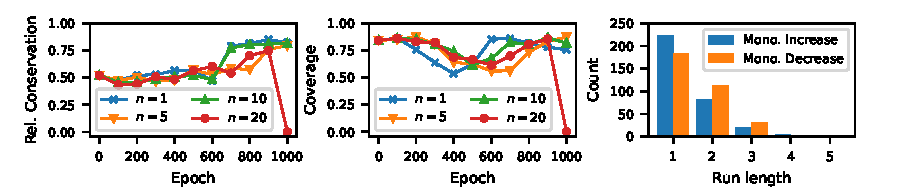
\includegraphics[scale=1.1]{masked_mnz_plots/fig3/exploit2.pdf}
\end{tabular}
\caption{Left: relative conservation and coverage of $\mathcal{O}_{w/2}$ trained on a random sequence using $\mathcal{L}_{exploit}$ with varying no. sampled mutations $n$; Right: no. segments with monotonically changing priority scores at each segment length.}
\label{fig:3}
\end{figure}

\noindent Fig.~\ref{fig:3} (left) plots the relative conservation and coverage metrics obtained over $1000$ epochs with different number of sampled mutations $n \in \{1,5,10,20\}$ per training epoch. We observe that $\mathcal{L}_{exploit}$ consistently improves relative conservation as expected. When $n=20$, the optimizer finds the exploit mentioned in Section~\ref{sec:analysis} after $1000$ epochs, which causes both metrics to reach $0$. The resulting sketch selects no $k$-mers (i.e., $0$ coverage) and is trivially conserved when mutations are introduced (i.e., infinity conservation, manually set to $0$). Fig.~\ref{fig:3} (right) plots the number of segments with monotonically increasing/decreasing priority scores at each segment length. The longest segment with monotonically decreasing priority score is $4$, which is smaller than the syncmer offset $t=w/2=5$. This implies that all lowest scoring $k$-mers are found within the first $t-1$ positions of their respective windows and none are sub-sampled into the syncmer sketch. Appendix~\ref{app-mask:f} repeats this experiment for $t=6,7,8,9$ and yields the same pattern with their discovered exploits, thus confirming the existence of our theoretical scenario in Section~\ref{sec:metric} and the necessity of the GSS metric.

\subsubsection{The minimizer mask is a good default configuration.} Fig.~\ref{fig:4} (left) shows the scatter plot of all $2^w$ masked minimizers trained on \textsc{Btr4} using $\mathcal{L}_{gss}$ with $w=10$ and $k=15$, grouped by the number of $1$-entries in their masks. Similar experiments on \textsc{Btr1}, \textsc{Btr2} and \textsc{Btr3} are deferred to Appendix~\ref{app-mask:f}. We observe that the average GSS increases with the number of $1$-entries in all experiments, which implies that the minimizer mask is a good default choice. However, we also observe that there exist specific masks that perform better than the minimizer mask, thus justifying mask optimization in certain applications.

\subsubsection{Preventing repeated sampling in homopolymer-rich sequences.} One advantage of syncmers with $t>1$ is the ability to avoid repeated sampling of identical $k$-mers in homopolymer substrings (i.e., substrings with repeated submer patterns) \cite{edgar2021syncmers}. To confirm this, Fig.~\ref{fig:4} (right) plots the GSS of all syncmer masks and their complements on a synthetic sequence with $L=100000$ and $0.2\%$ homopolymer content. The dotted line shows the GSS of the minimizer mask, which expectedly  performs worse than most syncmers (except for $t=1$) due to the repeated sampling pitfall. Because of the left-most tie breaking rule, every masked minimizers with a $1$ at the left most position of the mask (which includes minimizers, syncmers with $t$=1 and complement with $t \ne 1$) suffer from the pitfall of having a high density. This is indeed reflected in their similar GSS to the minimizer mask. On the contrary, we observe that the complement mask $\mathcal{C}_{1}$ (i.e., $1^{\text{st}}$ position is pruned) achieves the best GSS of $0.56$. This is because it avoids the repeated sampling pitfall in the same way any syncmer mask with $t>1$ does, but otherwise performs like a minimizer scheme and does not suffer from the low coverage of syncmers.

\begin{figure}[ht]
\centering
\begin{tabular}{c}
\hspace{-1.5mm}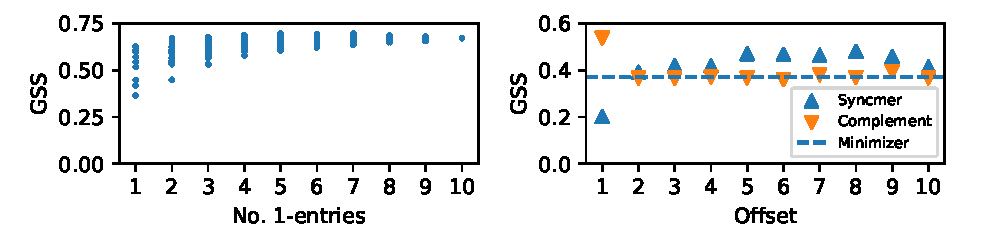
\includegraphics[scale=0.98]{masked_mnz_plots/fig4/exp78.pdf}
\end{tabular}
\caption{Left: GSS vs.\@ number of $1$-entries of all mask minimizers trained on the bacterial genome \textsc{Btr4}; Right: GSS vs.\@ offset positions of syncmer and complement masks on a synthetic sequence with high homopolymer content.}
\label{fig:4}
\end{figure}
